\CHAPTER{Appendix}
\label{chapter7}
\onehalfspace
\SECTION{Cavity stuff}
A pole-zero map of the cavity amplitude reflectivity transfer function is shown in Fig.\~ref{fig:cavpzmap}.

\begin{figure}[b]
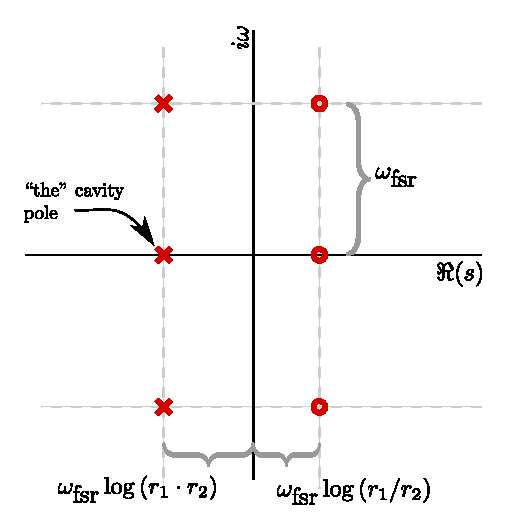
\includegraphics{figures/cavitypzmap.pdf}
\caption{\label{fig:cavpzmap} Pole-zero map of the cavity amplitude
  reflectivity.
  Poles are designated with $\times$ and zeros with
  $\circ$; $r_1$ is the amplitude reflectivity of the input coupler,
  and $r_2$ is the amplitude reflectivity of the output coupler.
  Losses can be lumped into $r_2$.  Notice that the free spectral
  range (angular frequency $\omega_{\textrm{fsr}}$) sets the scale of
  the entire diagram, and the function is periodic in $i\omega$: there
  is an infinite line of poles and an infinite line of zeros.  Two
  limiting cases are worth considering: (1) A critically-coupled
  cavity has $r_1=r_2$, which brings the line of zeros onto the
  imaginary axis. On resonance, $i\omega$ travels through these zeros
  and the cavity reflectivity vanishes.  This models the desired
  behavior of mode cleaner cavities. (2) A maximally over-coupled
  cavity has $r_2=1$, in which case the line of poles and line of
  zeros are equally spaced from the imaginary axis.  This models the
  LIGO arm cavities.  
  The cavity's amplitude transmission has the same poles as the
  reflectivity but no zeros.
}
\end{figure}

\SECTION{The difference between PM and AM}
\label{sec:am-vs-pm}
%
Suppose we have a signal consisting of a carrier (at frequency $\omega$ and
with unit amplitude) and two sidebands, of amplitudes $a$ (lower) and $b$
(upper), separated from the carrier by a frequency $\Omega$:
%
\begin{equation}
E(t) = \left(1 + a \exp(-i \Omega t) + b \exp(i \Omega t)\right)
\exp(i \omega t)
\end{equation}
%
To find the power in this signal, we take the
modulus squared, $P = E^*E$ where * is the complex conjugate:
%
\begin{equation}
\begin{split}
P = & \left(1 + |a|^2 + |b|^2\right) \\
    & + \left(a^* + b\right) \exp(-i \Omega t) + \left(a + b^*\right) \exp(i \Omega t) \\
    & + \left(ab^*\right) \exp(-2 i \Omega t) + \left(a^*b\right) \exp(2 i \Omega t)
\end{split}
\end{equation}
%
The condition for the $1\Omega$ variation in the power to vanish is
$a=-b*$, i.e. the real parts of the amplitudes of the sidebands must
be opposite, and the imaginary parts must be equal. So we can extract
the amplitude and phase modulation indicies:
%
\begin{equation}
\begin{split}
m_{AM} &= (a + b^*)\\
m_{PM} &= (a - b^*)
\end{split}
\end{equation}

What is the condition for the $2\Omega$ signal to vanish? With just
two sidebands, it will always be present (though at second order in
the sideband amplitude). In true phase modulation, the $2\Omega$
signal is cancelled by the interaction of (the infinite number of)
higher-order sidebands. As best I can tell, there is no simple
arrangement of this cancellation other than via a magical property of
the Bessel functions.

\SECTION{Only the signal field matters}

Suppose we have two electric fields incident on a photodiode: the
signal field $A_s$ and the local oscillator field $A_{LO}$.  The power
seen by the photodiode is
$$ \left| A_s + A_{LO} \right|^2 = 
   |A_s|^2 + |A_{LO}|^2 + 2 \mathrm{ Re } {A_s}^*A_{LO}$$
In the small-signal regime, $|A_s| << |A_{LO}|$.  The signal on the
photodiode is proportional to $A_s A_{LO}$ while the shot noise is
proportional to $\sqrt{|A_s|^2+|A_{LO}|^2}\approx A_{LO}$.  
  The detected SNR is independent of the local oscillator strength.

\SECTION{Optical phase conventions}
\SECTION{The optical spring}
\SECTION{Gaussian beams}
\SECTION{Laser modes}

The eigenmodes of an optical cavity formed from spherical lenses are
the Hermite-Gauss (if the cavity has rectangular symmetry) or
Laguerre-Gauss (for axial symmetry) modes.  The amplitude distribution
at the beam waist is a Gaussian multiplied by a Hermite or Laguerre
polynomial.  These are exactly the same familes of functions as the
energy eigenstate wavefunctions of the simple harmonic oscillator in
quantum mechanics.

\SECTION{Control theory basics}

Operation of the LIGO detectors relies crucially on feedback control
systems.  In general, the response of the optical plant is very
nonlinear; in order to produce a valid readout, the plant must be held
very close to its operating point.  The use of feedback control allows
us to attain linear response from an otherwise very nonlinear machine.

Here is a basic diagram of a feedback system:

Algebraically, one can derive a relationship giving the transfer function
of the closed-loop system in the Laplace domain:

\SECTION{The Antenna Pattern}

Gravitational waves come in two polarizations; for waves impinging
from a given direction, the second polarization represents an ellipse
of oscillating transverse strains rotated 45 degrees relative to the
first.  

Fundamentally, a Michelson interferometer is sensitive to two
polarizations of gravitational waves.  However, as seen in FIXME, we
elect to throw away sensitivity to one polarization in return for
common-mode noise immunity in the second polarization.

Although the waves come in two polarizations, one should note that
there is no globally consistent notion of \emph{the} $h_+$ and
$h_\times$ polarizations.  This is forbidden by the Hairy Ball
theorem.  

For a single detector, we can identify $h_+$ as the polarization
that shows up in DARM, and $h_\times$ as the polarization that would
show up in CARM.  Immediately (again due to the hairy ball theorem) we
see that there must be nulls in the sensitivity pattern of a single
interferometer.

\SECTION{Shot Noise}
The root-mean-square of a Poisson process with current $I$ and quantum
$q$ measured over a bandwidth of $\Delta f$ is 
$$\sigma = \sqrt{2 q I \Delta f}$$ 
Here $I$ could be the electric current in Amps (=Coulombs/second) and
$q$ the charge of an electron.  For light incident on a photodiode,
the photon shot noise can be considered as an energy current, with
$I\leftarrow P$ being the DC power, and $q\leftarrow h\nu$ being the
energy per photon.

The amplitude spectral density of this process is white, with
amplitude $\sqrt{2qI}$ in units of [I] per square root of Hz.

So, for power $P$, the shot noise amplitude spectral density is 
\begin{equation}
\text{shot noise ASD} = \sqrt{2 h\nu P}\quad [\text{Watts}/\sqrt{\text{Hz}]}
\label{eq:shotnoise-asd}
\end{equation}
for a relative intensity noise of $\sqrt{2 h\nu/P}$.

\SECTION{References}
\cite{Quetschke2007Complex}
